%\documentclass[a4paper]{article}
\usepackage[utf8]{inputenc}
\usepackage[spanish, es-tabla, es-noshorthands]{babel}
\usepackage[table,xcdraw]{xcolor}
\usepackage[a4paper, footnotesep=1.25cm, headheight=1.25cm, top=2.54cm, left=2.54cm, bottom=2.54cm, right=2.54cm]{geometry}
%\geometry{showframe}

%\usepackage{wrapfig}			%Wrap figure in text
\usepackage[export]{adjustbox}	%Move images
\usepackage{changepage}			%Move tables

\usepackage{tikz}
\usepackage{amsmath}
\usepackage{amsfonts}
\usepackage{amssymb}
\usepackage{float}
\usepackage{graphicx}
\usepackage{caption}
\usepackage{subcaption}
\usepackage{multicol}
\usepackage{multirow}
\usepackage{wrapfig}
\setlength{\doublerulesep}{\arrayrulewidth}
\usepackage{booktabs}
\usepackage[numbib, nottoc, notlot, notlof]{tocbibind}

\usepackage{hyperref}
\hypersetup{
    colorlinks=true,
    linkcolor=blue,
    filecolor=magenta,      
    urlcolor=blue,
    citecolor=blue,    
}

%Change Font Size

% #1 = size, #2 = text
\newcommand{\setparagraphsize}[2]{{\fontsize{#1}{6}\selectfont#2 \par}}		%Cambia el size de todo el parrafo
\newcommand{\setlinesize}[2]{{\fontsize{#1}{6}\selectfont#2}}				%Cambia el font de una oración

\newcommand{\note}[1]{
	\begin{center}
		\huge{ \textcolor{red}{#1} }
	\end{center}
}

%FONTS (IMPORTANTE): Compilar en XeLaTex o LuaLaTeX
\usepackage{anyfontsize}	%Font size
\usepackage{fontspec}		%Font type

\usepackage{etoolbox}
\usepackage{todonotes}

\newcommand{\observacion}[2]{  \ifnumequal{1}{#1}{ { \todo[inline,backgroundcolor=red!25,bordercolor=red!100]{\textbf{Observación: #2}} } }{  }  }

\setcounter{topnumber}{2}
\setcounter{bottomnumber}{2}
\setcounter{totalnumber}{4}
\renewcommand{\topfraction}{0.85}
\renewcommand{\bottomfraction}{0.85}
\renewcommand{\textfraction}{0.15}
\renewcommand{\floatpagefraction}{0.8}
\renewcommand{\textfraction}{0.1}
\setlength{\floatsep}{5pt plus 2pt minus 2pt}
\setlength{\textfloatsep}{5pt plus 2pt minus 2pt}
\setlength{\intextsep}{5pt plus 2pt minus 2pt}

\newcommand{\quotes}[1]{``#1''}
\usepackage{array}
\newcolumntype{C}[1]{>{\centering\let\newline\\\arraybackslash\hspace{0pt}}m{#1}}
\usepackage[american]{circuitikz}
\usetikzlibrary{calc}
\usepackage{fancyhdr}
\usepackage{units} 

\graphicspath{{../Control de posición no lineal/}{../Control de fuerza no lineal/}{../Control híbrido no lineal/}{../Referencias/}{../Deducción de modelo/}{../Conclusiones/}}

\pagestyle{fancy}
\fancyhf{}
\lhead{22.99 - Automación Industrial}
\rhead{Lambertucci, Londero B., Maselli, Mechoulam}
\rfoot{Página \thepage}

%Items con bullets y no cuadrados
\renewcommand{\labelitemi}{\textbullet }

%
%\begin{document}

\Subsection{Modelo Físico}
El doble péndulo invertido fue modelado como un manipulador Primático-Rotacional-Rotacional. 
\begin{figure}[H]
	\centering
	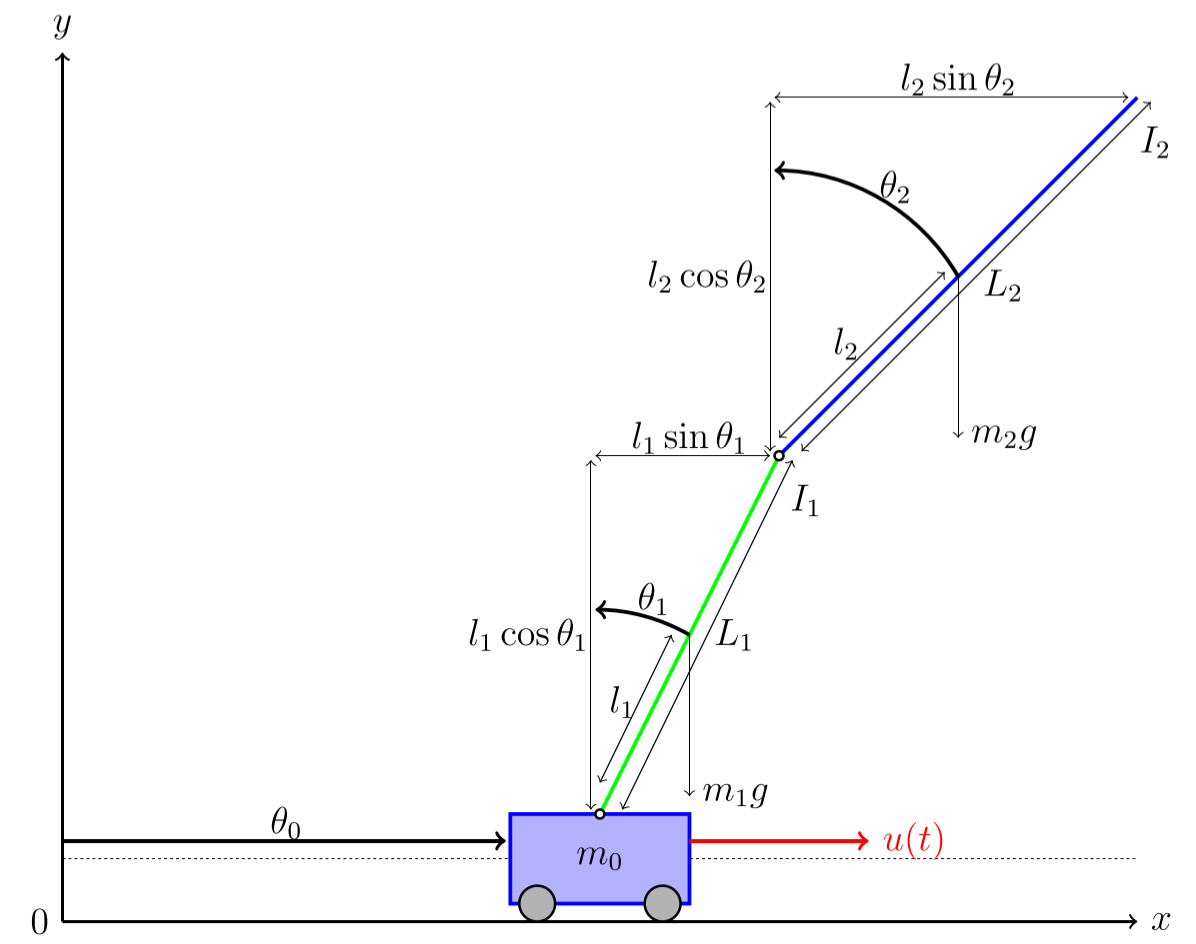
\includegraphics[width=\linewidth]{../Modelo Teorico/ImagenesModelo Teorico/sistema}
	\caption{Modelo teórico del doble péndulo invertido.}	
	\label{fig:pendteo}
\end{figure}
Luego utilizando la formulación de Euler-Lagrange.
\begin{equation}
  \frac{d}{dt}\frac{\partial L}{\partial \dot{\Theta}} - \frac{\partial L}{\partial \Theta}  = \tau
\end{equation} 
\begin{equation}
L\left( \Theta , \dot{\Theta} \right) = \sum_{i=0}^2
\left( \frac{1}{2} m_i v_{Ci}^Tv_{Ci} +\frac{1}{2} I_i \omega_{Ci}^T\omega_{Ci} + u_{refi} - m_i g d_{Ci}\right)
\end{equation} 
Se llega al sistema de segundo orden no lineal:
\begin{equation}
\tau = M\left( \Theta \right)\ddot{\Theta} + V\left( \Theta , \dot{\Theta} \right) + G\left( \Theta \right)
\end{equation}
Siendo las matrices:
\begin{equation}
 M\left( \Theta \right)\ddot{\Theta} = \begin{bmatrix}
m_0+m_1+m_2 & \left( m_1l_1 + m_2L_1 \right) \cos \theta_1 & m_2l_2 \cos \theta_2\\

\left( m_1l_1 + m_2L_1 \right) \cos \theta_1  &
m_1l_1^2+m_2L_1^2+I_1
& m_2L_1l_2\cos(\theta_1-\theta_2)\\


m_2l_2\cos\theta_2 & m_2L_1l_2\cos(\theta_1-\theta_2) & m_2l_2^2+I_2
\end{bmatrix}
\end{equation}
\begin{equation}
 V\left( \Theta , \dot{\Theta} \right) =
 \begin{bmatrix}
0 & -\left( m_1l_1 + m_2L_1 \right)\sin \theta_1 \dot{\theta_1} & -m_2l_2\sin \theta_2 \dot{\theta_2}\\
0 & 0 & m_2L_1l_2\sin(\theta_1-\theta_2)\dot{\theta_2}\\
0 & -m_2L_1l_2\sin(\theta_1-\theta_2)\dot{\theta_1} & 0
\end{bmatrix}
\end{equation}
\begin{equation}
 G\left( \Theta \right) = \begin{bmatrix}
0 \\
 -(m_1l_1+m_2L_1)g\sin\theta_1 \\
-m_2gl_2\sin\theta_2
\end{bmatrix}
\end{equation}
\begin{equation}
 H = \begin{bmatrix}
1 \\
 0 \\
0
\end{bmatrix}
\hspace{1cm}
\tau = H\cdot u(t)
\end{equation}
Si se asume los siguientes valores:
\begin{equation}
l1 = \frac{1}{2} L_1
\hspace{1cm}
l2 = \frac{1}{2} L_2 
\hspace{1cm}
I_1 = \frac{1}{12} m_1L_1^2
\hspace{1cm}
I_2 = \frac{1}{12} m_2L_2^2
\end{equation}
Se simplifica a :
\begin{equation}
 M\left( \Theta \right)\ddot{\Theta} = \begin{bmatrix}
m_0+m_1+m_2 & \left( \frac{1}{2}m_1L_1 + m_2 \right) L_1\cos \theta_1  \frac{1}{2}& m_2L_2 \cos \theta_2\\

\left(  \frac{1}{2}m_1 + m_2 \right) L_1 \cos \theta_1  &
\left( \frac{1}{3}m_1+m_2\right) L_1^2
&  \frac{1}{2}m_2L_1L_2\cos(\theta_1-\theta_2)\\


 \frac{1}{2}m_2L_2\cos\theta_2 &  \frac{1}{2}m_2L_1L_2\cos(\theta_1-\theta_2) &  \frac{1}{3}m_2L_2^2
\end{bmatrix}
\end{equation}
\begin{equation}
 V\left( \Theta , \dot{\Theta} \right) =
 \begin{bmatrix}
0 & -\left(  \frac{1}{2}m_1 + m_2\right)L_1\sin \theta_1 \dot{\theta_1} & - \frac{1}{2}m_2L_2\sin \theta_2 \dot{\theta_2}\\
0 & 0 &  \frac{1}{2}m_2L_1L_2\sin(\theta_1-\theta_2)\dot{\theta_2}\\
0 & - \frac{1}{2}m_2L_1L_2\sin(\theta_1-\theta_2)\dot{\theta_1} & 0
\end{bmatrix}
\end{equation}
\begin{equation}
 G\left( \Theta \right) = \begin{bmatrix}
0 \\
 - \frac{1}{2}(m_1+m_2)L_1g\sin\theta_1 \\
- \frac{1}{2}m_2gL_2\sin\theta_2
\end{bmatrix}
\end{equation}
\begin{equation}
 H = \begin{bmatrix}
1 \\
 0 \\
0
\end{bmatrix}
\hspace{1cm}
\tau = H\cdot u(t)
\end{equation}
Cabe mencionar que $M(\Theta)$ es una matriz simétrica no-singular, por lo que existe la inversa y también es simétrica.

%\end{document}
